\newcommand{\department}{Физики}
\newcommand{\labnum}{2}
\newcommand{\discipline}{Физика}
\newcommand{\theme}{ИССЛЕДОВАНИЕ ИНТЕГРАЛЬНЫХ ХАРАКТЕРИСТИК ЭЛЕКТРОСТАТИЧЕСКОГО ПОЛЯ МЕТОДОМ МОДЕЛИРОВАНИЯ (циркуляция напряженности)}
\newcommand{\haspartner}{0} % 0 or 1
\newcommand{\partnername}{} % Миллер В.В.
\newcommand{\teachername}{Чурганова С.С.} % Кузьмин С.А.
\newcommand{\labyear}{2020}

\documentclass[12pt,a4paper]{article}  % шаблон для статьи, шрифт 12 пт

\usepackage[utf8]{inputenc}  % использование кодировки Юникод UTF-8
\usepackage[T1]{fontenc}
\usepackage[russian]{babel}  % пакет поддержки русского языка

\usepackage{indentfirst}  % отступ первого абзаца
\setlength{\parindent}{0.75cm}

\usepackage{amsmath}

\usepackage[compact]{titlesec}  % для titlespacing
% \titlespacing{\заголовок}{слева}{перед}{после}[справа]
\titlespacing*{\section}{0.75cm}{1em}{0.1em}  % отступ заголовка
\titlespacing*{\subsection}{0.75cm}{1em}{0.1em}


\usepackage{graphicx}  % кртинки
\usepackage{float} % плавающие картинки
\usepackage{wrapfig}  % Обтекание фигур (таблиц, картинок и прочего)
\usepackage[labelsep=endash]{caption}  % тире вместо двоеточия в картинках
\usepackage{amsmath}





\begin{document}

	\thispagestyle{empty}

\begin{center}
    \Large{
    \textbf{МИНОБРНАУКИ РОССИИ}

    \textbf{Санкт-Петербургский государственный}

    \textbf{электротехнический университет «ЛЭТИ»}

    \textbf{им. В.И. Ульянова (Ленина)}

    \textbf{Кафедра \department}
    }
\end{center}

\topskip=0pt
\vspace*{\fill}

\begin{center}
    \Large{
    \textbf{
    Решения задач ИДЗ №3\\
    по дисциплине «\discipline»\\
    Вариант 9\\
    }
    }
\end{center}

\vspace*{\fill}

\begin{tabular}{lcr}
    Студент\if \haspartner 1 ы \fi гр. 9892 & \begin{tabular}{p{60mm}} \\ \hline \end{tabular} & Лескин К.А.  \\\\
    \if \haspartner 1
                      & \begin{tabular}{p{60mm}} \\ \hline \end{tabular} & \partnername \\\\
    \fi
    Преподаватель     & \begin{tabular}{p{60mm}} \\ \hline \end{tabular} & \teachername
    \\\\
\end{tabular}

\begin{center}
    Санкт-Петербург\\
    \labyear
\end{center}

\newpage
	
	\section*{Цель}

Экспериментальное исследование зависимости полезной
мощности, полной мощности и коэффициента полезного действия (КПД)
источника от отношения сопротивлений нагрузки и источника. 
	
	\section*{Приборы и принадлежности}

Стенд для сборки измерительной цепи; два
источника с различными ЭДС; миллиамперметр и вольтметр; переменный
резистор. 
	
	\newpage
	
	\section*{Исследуемые закономерности}

В лабораторной работе измеряется магнитное поле земли 
на основе явления электромагнитной индукции.

При повороте контура, состоящего из $ N $ витков, в однородном магнитном поле с
индукцией $ В $ в нем наводится электродвижущая сила (ЭДС) электромагнитной индукции 

\begin{equation}
	E_i = -\dfrac{d\Psi}{dt}
\end{equation}

$ \Psi = N\Phi $ -- полный магнитный поток (потокосцепление), сцепленный с контуром;

$ \Phi = BS\cos{\alpha} $ -- поток вектора В через плоскую поверхность площадью S,
охватываемую контуром;

$ S = Sn $ -- вектор, равный $ S $ по модулю и направленный по
нормали к этой поверхности;

$ n $ -- орта нормали;

$ \alpha $ -- угол между векторами $ В $ и $ n $.
 
В работе устоновка расположена так, что $ \alpha = 0 $.

ЭДС, возникающая при повороте контура вызывает индукционный ток, переносящий заряд 
через поперечное сечение проводников контура.

В итоге получаем напряжение

\begin{equation}\label{key}
	U = \dfrac{2NBS}{RC}
\end{equation}
	
	\section*{Протокол}


	
	\section*{Обработка результатов измерений}

Рассчитаем вектор напряжённости:

$ 
E = \dfrac{d\varphi}{dl} = 
\dfrac{\varDelta \varphi}{\varDelta l}
$\\

$ 
\overline E_x =
\dfrac{\varDelta \varphi}{\varDelta x} =
\dfrac{5.55 - 5.52}{0.005} =
6 \dfrac{B}{m}
$\\

$ 
\overline E_y =
\dfrac{\varDelta \varphi}{\varDelta y} =
\dfrac{5.53 - 5.52}{0.005} =
2 \dfrac{B}{m}
$\\

Рассчитаем погрешность вектора напряжённости:

$ 
\varDelta E = 
\dfrac{\varphi_1 - \varphi_2}{x_1 - x_2}
$\\

$ 
\varDelta E_x = 
\sqrt{
    2(\dfrac{\theta_\varphi}{\varDelta x})^2 + 
    2(\dfrac{\varDelta \varphi \theta_l}{\varDelta x ^2})^2
} = 
\sqrt{
    2(\dfrac{0.01}{0.005})^2 + 
    2(\dfrac{0.03 * 0.001}{0.000025})^2
} = 
3,3
$\\

$ 
\varDelta E_y = 
\sqrt{
    2(\dfrac{\theta_\varphi}{\varDelta y})^2 + 
    2(\dfrac{\varDelta \varphi \theta_l}{\varDelta y ^2})^2
} = 
\sqrt{
    2(\dfrac{0.01}{0.005})^2 + 
    2(\dfrac{0.03 * 0.001}{0.000025})^2
} = 
2,9
$\\

$ 
E = 
\sqrt{
    E_x^2 + E_y^2 
} = 6.3 \pm 4.3
$\\

Рассчитаем касательные составляющие для отрезков выбранного контура:\\ 

% E 1 #########################
$
E_{1} = 
\dfrac{\varDelta \varphi}{\varDelta l} =
\dfrac{7.31 - 7.01}{0.004} = 
75.0
$\\


% E 2 #########################
$
E_{2} = 
\dfrac{\varDelta \varphi}{\varDelta l} =
\dfrac{7.73 - 7.5}{0.004} = 
57.5
$\\


% E 3 #########################
$
E_{3} = 
\dfrac{\varDelta \varphi}{\varDelta l} =
\dfrac{8.02 - 7.98}{0.004} = 
10.0
$\\


% E 4 #########################
$
E_{4} = 
\dfrac{\varDelta \varphi}{\varDelta l} =
\dfrac{8.16 - 8.18}{0.004} = 
-5.0
$\\


% E 5 #########################
$
E_{5} = 
\dfrac{\varDelta \varphi}{\varDelta l} =
\dfrac{8.06 - 8.25}{0.004} = 
-47.5
$\\


% E 6 #########################
$
E_{6} = 
\dfrac{\varDelta \varphi}{\varDelta l} =
\dfrac{8.0 - 8.12}{0.004} = 
-30.0
$\\


% E 7 #########################
$
E_{7} = 
\dfrac{\varDelta \varphi}{\varDelta l} =
\dfrac{7.77 - 7.94}{0.004} = 
-42.5
$\\


% E 8 #########################
$
E_{8} = 
\dfrac{\varDelta \varphi}{\varDelta l} =
\dfrac{7.44 - 7.69}{0.004} = 
-62.5
$\\


% E 9 #########################
$
E_{9} = 
\dfrac{\varDelta \varphi}{\varDelta l} =
\dfrac{7.04 - 7.25}{0.004} = 
-52.5
$\\


% E 10 #########################
$
E_{10} = 
\dfrac{\varDelta \varphi}{\varDelta l} =
\dfrac{6.65 - 6.95}{0.004} = 
-75.0
$\\


% E 11 #########################
$
E_{11} = 
\dfrac{\varDelta \varphi}{\varDelta l} =
\dfrac{6.53 - 6.55}{0.004} = 
-5.0
$\\


% E 12 #########################
$
E_{12} = 
\dfrac{\varDelta \varphi}{\varDelta l} =
\dfrac{6.2 - 6.44}{0.004} = 
-60.0
$\\


% E 13 #########################
$
E_{13} = 
\dfrac{\varDelta \varphi}{\varDelta l} =
\dfrac{6.14 - 6.17}{0.004} = 
-7.5
$\\


% E 14 #########################
$
E_{14} = 
\dfrac{\varDelta \varphi}{\varDelta l} =
\dfrac{6.04 - 6.1}{0.004} = 
-15.0
$\\


% E 15 #########################
$
E_{15} = 
\dfrac{\varDelta \varphi}{\varDelta l} =
\dfrac{6.04 - 6.17}{0.004} = 
-32.5
$\\


% E 16 #########################
$
E_{16} = 
\dfrac{\varDelta \varphi}{\varDelta l} =
\dfrac{6.13 - 6.08}{0.004} = 
12.5
$\\


% E 17 #########################
$
E_{17} = 
\dfrac{\varDelta \varphi}{\varDelta l} =
\dfrac{6.63 - 6.47}{0.004} = 
40.0
$\\


% E 18 #########################
$
E_{18} = 
\dfrac{\varDelta \varphi}{\varDelta l} =
\dfrac{6.91 - 6.81}{0.004} = 
25.0
$\\

\begin{figure}
    \centering
    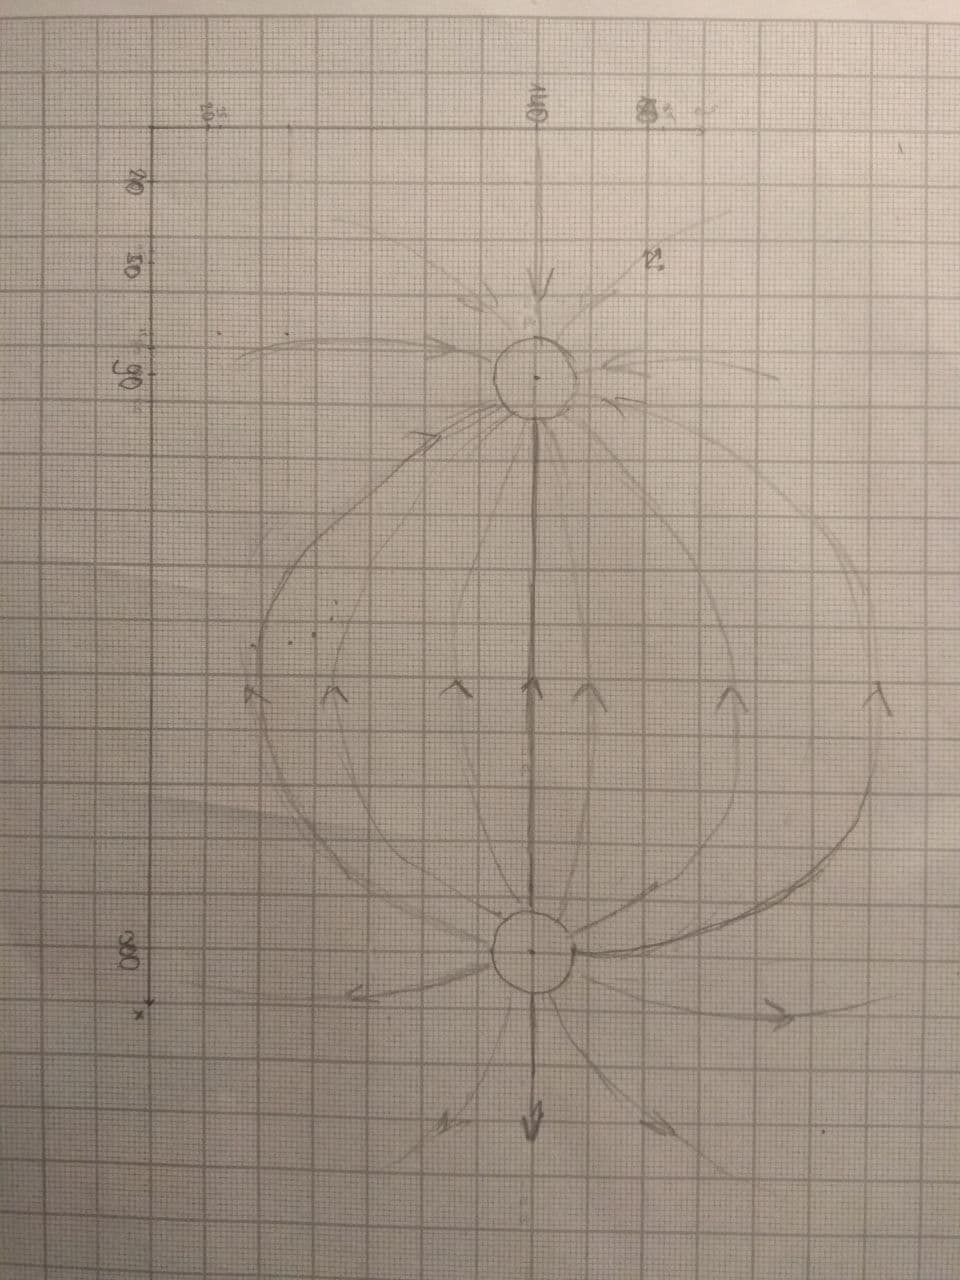
\includegraphics[width=\linewidth,angle=180]{photo/s}
\end{figure}




	
	\section*{Вывод}

В ходе выполнения лабораторной работы было изучено действие магнитного поля на движущиеся заряды в полупроводнике, 
с электронным типом проводимости, 
определена постоянной Холла, 
концентрация и подвижность носителей
заряда. 

\end{document}